\chapter{The micromagnetic model}
In this thesis we will base our work on the micromagnetic model. This model is a semi-classical theory that is conventionally used to describe both the equilibrium and dynamics of the magnetization in a material on a nanometer to micrometer length scale. This length scale is large enough to assume a continuum approximation, we can consider the magnetization as a smooth and continuously varying vector field in space, as it is greater than the typical atomic length scale. On this length scale it is also not necessary to do a full quantum mechanical treatment of the system, making it justifiable to primarily treat quantities as expectation values instead of operators. The length scale is small enough, however, to be able to successfully describe patterns in the magnetization that are observed in nature, such as magnetic domain walls and magnetic skyrmions. This model is also able to describe the motion of such magnetization patterns well, which makes it a highly attractive model in the field of magnetization dynamics.
%\section{Zeeman energy}
%The Zeeman energy is the energy contribution from the interaction between the magnetization $\mathbold{M}(\mathbold{r})$ in the magnetic material and an external magnetic field $\mathbold{H}_{\text{Z}}(\mathbold{r})$. This energy can be expressed as
%\begin{align}
%E_{\text{Z}} = -\mu_0\int \d V \mathbold{M}(\mathbold{r})\cdot\mathbf{H}_{\text{Z}}(\mathbold{r}),
%\end{align}
%with $\mu_0$ being the vacuum permeability.
\section{Energy terms in micromagnetics}
In conventional micromagnetics there are five contributions to the micromagnetic energy. These are the exchange energy, the anisotropic energy, the Zeeman energy, the demagnetization energy, and the magneto-elastic energy. Of these five energies we will only discuss the former three. The demagnetization energy is not considered as it is mainly dominant over larger length scales, and the length scale that we will primarily consider is on the nanometer length scale. The magneto-elastic energy is also neglected, as we will not consider elastic distortion of the lattice. We will, however, also consider energy contributions that are not included in conventional micromagnetics, such as the Ruderman--Kittel--Kasuya--Yosida interaction, Rashba spin--orbit coupling, the Dzyaloshinskii--Moriya interaction and pinning potentials. We will treat these energy contributions in the same manner, assuming a continuum model of the magnetization if applicable (the Ruderman--Kittel--Kasuya--Yosida interaction for example is an interaction between discrete magnetic moments, and a continuum model is therefore not suitable).
\subsection{Exchange energy} \label{sec:Exchange}
Ferromagnetism occurs in materials where the spins tend to align with each other, and thereby being able to generate an observable magnetic field outside of the material. The mechanism behind this is the exchange interaction between the spins. In ferromagnetic materials the system can lower its energy by having parallel neighboring spins. This is described by the Heisenberg Hamiltonian,
\begin{align}
H = - J\sum_{\langle i,j\rangle} \mathbold{S}_i\cdot\mathbold{S}_j,
\end{align}
with $J$ being the exchange integral which is positive for ferromagnetic materials and $\mathbold{S}$ a dimensionless spin-vector. The spins can be expressed in terms of the magnetization, which is the average magnetic moment. As the magnetic moment and the spin of an electron are anti-parallel, this relation becomes
\begin{align}
\label{eq:ExchangeHamiltonian}
\mathbold{S}_i = -\frac{S}{M_s}\mathbold{M}_i,
\end{align}
with $M_s$ being the saturation magnetization and $S$ the magnitude of the spin. The magnetization is a classical vector, and in micromagnetism it is treated as a slowly varying smooth function. One can therefore perform a Taylor expansion of it. By doing that, one can show \cite{Project} that the energy density can be written as
\begin{align}
\epsilon_{\text{EX}} = \frac{\textrm{d} E_{\text{EX}}}{\textrm{d} V} = -\frac{A}{M_s^2}\mathbold{M}(\mathbold{r})\mathbold{\nabla}^2\mathbold{M}(\mathbold{r}) = \frac{A}{M_s^2}\partial_i\mathbold{M}(\mathbold{r})\partial_i\mathbold{M}(\mathbold{r}), \label{eq:exchDensity}
\end{align}
with $A$ being the exchange stiffness
\begin{align}
A = \frac{J S^2}{2a}
\end{align}
and $a$ being the lattice constant.

\subsection{Zeeman energy}
When turning on an external magnetic field in a magnetic material, the magnetic moments in the material tend to align with the magnetic field. This is due to the Zeeman interaction, which will go to a lower energy state if the magnetic moments and external field are aligned. The Zeeman interaction energy density is given by
\begin{align}
\epsilon_{\text{Z}} = -\mu_0 \mathbold{M}\cdot\mathbold{H}_{\text{Z}},
\end{align}
with $\mathbold{H}_{\text{Z}}$ being the external magnetic field.

\subsection{Perpendicular magnetic anisotropy} \label{sec:PMA}
In some magnetic materials we may have something known as magnetic anisotropy. As the name indicates, there is an anisotropy in the material that makes certain magnetization directions more energetically favorable than others. This mostly stems from the spin--orbit coupling. If one considers the rest frame of the electron instead of the proton, the proton is orbiting the electron and thereby causing a temporally varying electric field. Amp\`{e}re's circuital law then says that the electron observes a magnetic field proportional to the orbital motion of the proton. This magnetic field then interacts with the magnetic moment (proportional to the spin) of the electron like in the Zeeman interaction, except here due to internal fields, hence the name spin--orbit coupling. Taking this into consideration as well as the atomic structure in the material, one can see that one could end up with a material where the magnetic field the electrons experience from the spin--orbit coupling would allow one direction to be easier magnetized than others.

In some layered ultrathin film structures, such as Pd/Co \cite{Carcia1985}, it has been discovered that the magnetization has a lower energy when it is perpendicular to the films. This means that the easy axis of the material is perpendicular to the films, and we then have something called perpendicular magnetic anisotropy (PMA). The anisotropic energy is independent of the direction the magnetization has along the easy axis, meaning the energy is the same if the magnetization points into or out of the films. Letting $K$ be the anisotropy constant and $\theta$ the angle to the normal of the films, the anisotropic energy density can then be written as
\begin{align}
\epsilon_{\text{PMA}} = K\sin^2\theta \label{eq:PMADensity}
\end{align} 
to the lowest order in $\theta$. Here we have normalized the energy density in such a way that if the magnetization points along the easy axis the energy density is zero.

\subsection{Voltage induced magnetic anisotropy} \label{sec:VIMA}
One form of perpendicular magnetic anisotropy occurs at the interface between certain materials. This has been attributed to the exchange interaction between $p$- and $d$-oribitals at material interfaces, such as the 3$d$ orbital in Fe and 2$p$ orbital in O at an Fe/MgO interface \cite{Matsukura2015}. As this is a magnetic anisotropy that only occurs at the surface of the material, it will only be of importance in ultra-thin magnetic films where surface effects are of a greater importance. It has also been discovered that one can modify the strength of this surface magnetic anisotropy with an external electric field. The reason for the change of strength in the magnetic anisotropy is the modification of the occupation number in the 3$d$ orbitals in Fe, thereby affecting the $p$-$d$ exchange interaction that is the origin of the magnetic surface anisotropy \cite{Maruyama2009}. It was found that in a thin-film system with an Fe/MgO interface where the Fe layer consisted of only a few monoatomic layers a change of approximately 40\% could be achieved in the magnetic surface anisotropy by application of an external electric field. As it is relatively easy to generate a localized electric field, one can therefore create an energy landscape to influence the dynamics of magnetization patterns. An example of this was shown by Upadhyaya \etal~by guiding dipole-dipole interaction skyrmions with voltage gates \cite{Upadhyaya2015}.

As the voltage induced magnetic anisotropy behaves as PMA, the energy density must then have the same form as that of $\epsilon_{\text{PMA}}$ in \eqref{eq:PMADensity} and be dependent on the electric field. If one assumes that the modification of the electric field on the PMA is linear in the electric field, the energy density can be written as
\begin{align}
\epsilon_{\text{EF}} = \eta E(\mathbold{r}) \sin^2\theta,
\end{align}
where $\eta$ is a materialistic constant describing the strength of the modification of PMA by the electric field, and the electric field strength $E(\mathbold{r})$ is the $z$-component of the electric field as a function of position in the thin film. 

\subsection{Ruderman--Kittel--Kasuya--Yosida interaction}
In metals, there is also another type of exchange interaction between magnetic moments in addition to the one described in Section \ref{sec:Exchange}. This interaction between nuclear magnetic moments is an indirect interaction. First a conduction electron in the atom interacts with the nuclear magnetic moment (proportional to its spin) through the hyperfine interaction. The hyperfine interaction is similar to the spin--orbit coupling discussed in Section \ref{sec:PMA}. Instead of being in the rest frame of the electron, however, we consider the magnetic field seen in the rest frame of the nucleus due to the orbital motion of the electron. In addition, as the electron carries with it an intrinsic magnetic moment, it will generate a magnetic field that will interact with the spin of the nucleus. In short, the hyperfine interaction consists of spin--orbit and spin--spin interactions seen from the rest frame of the nucleus. Going back to the conduction electron that has interacted with the nuclear magnetic moment through the hyperfine interaction, it can also interact with another nuclear magnetic moment after interacting with the first. It can therefore act as a mediating particle for the interaction between the magnetic moments of two different nuclei. This interaction is known as the Ruderman--Kittel--Kasuya--Yosida (RKKY) interaction \cite{RudermanKittel1954, Kasuya1956, Yosida1957, Vleck1962}, and its Hamiltonian is given by
\begin{align}
    \label{eq:RKKYHamiltonian_old}
    H_{\text{RKKY}} = \frac{\mathbold{I}_i\cdot\mathbold{I}_j}{4}\frac{|\Delta k_m k_m|^2m^*}{(2\pi)^3 R_{ij}^4 \hbar^2} \left[2k_mR_{ij}\cos\left(2k_mR_{ij}\right) - \sin \left(2k_mR_{ij}\right)\right].
\end{align}
Here $\mathbold{I}_i$ and $\mathbold{I}_j$ are the nuclear magnetic moments, $R_{ij}$ the distance between the magnetic moments, $k_m$ the wave number of the conduction electrons, $m^*$ the effective mass of the electrons and $\Delta k_m k_m$ is a factor describing the strength of the hyperfine interaction. What is important to note here is that the RKKY Hamiltonian acts similarly to the exchange Hamiltonian \eqref{eq:ExchangeHamiltonian} in a manner that it is a symmetric interaction between spins, and that the coupling strength between the spins is a function of distance. Moreover, unlike the exchange interaction, this function of distance can either be positive or negative depending on the value of $k_mR_{ij}$. This means that we can alter if two magnetic moments are ferromagnetically or antiferromagnetically coupled to each other by increasing or decreasing the distance between them. The way the interaction is formulated in \eqref{eq:RKKYHamiltonian_old} it is between two nuclear magnetic moments. However, the RKKY  interaction can also occur in a multilayer system such as F$_1$/N/F$_2$ where F$_i$ are thin uniformly magnetized magnetic metals and N is a non-magnetic metallic spacer, as shown by Parkin and Mauri in \cite{Parkin1991}. If one lets the magnetization in F$_i$ be $\mathbold{M}_i$, the RKKY interaction energy in F$_i$ can then be written as
\begin{align}
    H_{\text{RKKY}} = -\frac{J_{\text{RKKY}}(R_{ij})}{d_iM_s^2}\mathbold{M}_i\cdot\mathbold{M}_j,
\end{align}
with $J_{\text{RKKY}}(R_{ij})$ being the distance dependent coupling strength between the magnetic moments that can be both positive and negative, and $d_i$ being the thickness of F$_i$. The magnetic layers will then have a ferromagnetic coupling when $J_{\text{RKKY}}>0$ and an antiferromagnetic coupling when $J_{\text{RKKY}}<0$.

\subsection{The Rashba effect}
In materials where the motion of the electrons is confined to a plane, and the inversion symmetry is broken along the axis perpendicular to that plane, there is a splitting of the spin energy levels. Inversion symmetry can for example be broken at the interface between two materials \cite{Heide2006}. The inversion asymmetry causes an electric field perpendicular to the plane of motion, as the gradient of the electrostatic potential becomes non-zero when inversion symmetry is broken ($V(\mathbold{r}) \neq V(-\mathbold{r})$). When particles move in an electric field, they experience a magnetic field which can be seen by performing a Lorentz transformation into the particles' restframe. This magnetic field is proportional to $\mathbold{v}\times\mathbold{E}$. Because of the magnetic field the energy levels become spin dependent, as the field couples to the spin. This is described by the Rashba Hamiltonian \citep{BychovRashba1984}
\begin{align}
H_{\text{R}} &= \frac{\alpha_{\text{R}}}{\hbar}\mathbold{\sigma}\cdot(\mathbold{p}\times\mathbold{\hat{n}}) = \alpha_{\text{R}} (\mathbold{\sigma}\times\mathbold{k})\cdot\mathbold{\hat{n}}.
\label{eq:RashbaH}
\end{align}
Here $\alpha_{\text{R}}$ is the Rashba parameter, $\mathbold{p} = \hbar\mathbold{k}$ the momentum of the electrons, $\mathbold{\hat{n}}$ a unit vector perpendicular to the plane of motion (along the direction of broken inversion symmetry) and $\mathbold{\sigma}$ is a vector of the Pauli matrices. This can be seen as the magnetic field points along the direction $\mathbold{v}\times\mathbold{E}$, and as $\mathbold{p}\propto\mathbold{v}$ and $\mathbold{E}$ points along the direction of broken inversion symmetry given by $\mathbold{\hat{n}}$, the magnetic field therefore points along $\mathbold{p}\times\mathbold{\hat{n}}$. According to the Zeeman energy the energy should be then proportional to $\mathbold{\sigma}\cdot(\mathbold{p}\times\mathbold{\hat{n}})$, and this proportionality constant is given by $\alpha_{\text{R}}$, the value of which contains the physics of the broken inversion symmetry. This effect is a form of spin--orbit interaction, as the spin of the electron ($\propto \mathbold{\sigma}$) interacts with its own motion ($\mathbold{v}$). This effect is therefore also called Rashba spin--orbit coupling (RSOC).

\subsection{The Dzyaloshinskii--Moriya interaction}
The Dzyaloshinskii--Moriya interaction (DMI) is an antisymmetric exchange coupling between spins, given by the Hamiltonian
\begin{align}
H_{\text{DM}} = \sum_{\langle i,j\rangle}\mathbold{D}_{ij}\cdot(\mathbold{S}_i\times\mathbold{S}_j). \label{eq:DMIHamiltonian}
\end{align}
This interaction only occurs in materials where the inversion symmetry is broken. The magnitude of $\mathbold{D}_{ij}$ depends on the material properties, and the direction of $\mathbold{D}_{ij}$ depends on the symmetry of the atomic structure in the material. Moriya showed \cite{Moriya1960} that if there is an $n$-fold axis (with $n \geq 2$) along the axis between the particles with spins $\mathbold{S}_i$ and $\mathbold{S}_j$, $\mathbold{D}_{ij}$ will be parallel to that axis. Using that in a Taylor expansion of \eqref{eq:DMIHamiltonian}, it can be shown \cite{Project} that the energy density becomes
\begin{align}
\label{eq:DMBulk}
\epsilon_{\text{DM}}^{\textrm{(bulk)}} = \frac{D}{M_s^2}\mathbold{M}\cdot(\mathbold{\nabla}\times\mathbold{M}).
\end{align}
On the other hand, if there is a mirror plane located at the center of the line between the particles with spins $\mathbold{S}_i$ and $\mathbold{S}_j$ that is perpendicular to the axis intersecting them, the vector $\mathbold{D}_{ij}$ lies in the mirror plane. In a more specific case where the interaction between the spins $\mathbold{S}_i$ and $\mathbold{S}_j$ is mediated by a third magnetic particle (different from the other two) located in the mirror plane, $\mathbold{D}_{ij}$ is perpendicular to the triangle spanned by the three particles as illustrated in Figure \ref{fig:InterfacialDMI}. 
%\begin{figure}[h!]
%\begin{center}
%\includegraphics[width=0.6\textwidth]{Figures/InterfacialDMI.pdf} 
%\caption{An illustration of the geometry of an interfacial DMI. The antisymmetric interaction between the spins $\mathbold{S}_i$ and $\mathbold{S}_j$ is mediated by a third magnetic particle in blue. The direction of $\mathbold{D}_{ij}$ is then perpendicular to the plane spanned by the three particles.}
%\label{fig:InterfacialDMI} 
%\end{center}
%\end{figure}
\begin{figure}[h!]
\centering
\begin{tikzpicture}
\node[above right] (img) at (0,0) {\includegraphics[width=0.6\textwidth]{Figures/InterfacialDMIv2}};
\node at (70pt,110pt) {\Large{$\mathbold{S}_i$}};
\node at (210pt,110pt) {\Large{$\mathbold{S}_j$}};
\node at (140pt,10pt) {\Large{$\pm\mathbold{D}_{ij}$}};
\end{tikzpicture}
        \caption{An illustration of the geometry of an interfacial DMI. The antisymmetric interaction between the spins $\mathbold{S}_i$ and $\mathbold{S}_j$ is mediated by a third magnetic particle in blue. The direction of $\mathbold{D}_{ij}$ is then perpendicular to the plane spanned by the three particles.}
        \label{fig:InterfacialDMI}
\end{figure}
We now assume that the magnetic particles with spins $\mathbold{S}_i$ and $\mathbold{S}_j$ are located in the $xy$-plane, and that the mediating magnetic particle of a different type lies above them. According to symmetry, the vector $\mathbold{D}_{ij}$ is then given by $\mathbold{D}_{ij} = D/a\mathbold{\hat{y}}$ if $i$ and $j$ are nearest neighbours in the $x$-direction, and $\mathbold{D}_{ij} = -D/a\mathbold{\hat{x}}$ if $i$ and $j$ are nearest neighbours in the $y$-direction. Here $a$ is the lattice constant and $D$ a constant that can be both positive and negative. We have for simplicity assumed an equal interaction in all directions in the $xy$-plane. Using this result, we explicitly derive the expression for the interfacial DMI energy density for reasons we will see in Section \ref{sec:Parity}. As the spin can be written in terms of the magnetization as $\mathbold{S} = -\mathbold{M}S/M_s$, the Dzyaloshinskii--Moriya Hamiltonian can be written as
\begin{align}
    H_{\text{DM}} = \frac{1}{M_s^2}\sum_{\langle i,j\rangle} \mathbold{D}_{ij}\cdot\left( \mathbold{M}_i\times\mathbold{M}_j\right)
\end{align}
where the $S^2$ has been included in the magnitude of $\mathbold{D}_{ij}$. As mentioned earlier, we can do a Taylor expansion of the magnetization as it is a continious function in the micromagnetic model. To first order this Taylor expansion becomes
\begin{align}
    \mathbold{M}_{i+1} \approx \mathbold{M}_i + a\frac{\partial\mathbold{M}_i}{\partial x}
\end{align}
in the $x$-direction. An entirely equivalent expansion can also be done in the $y$-direction. The expansion in the $z$-direction is ignored as $\mathbold{D}_{ij}$ does not have a $z$-component. The energy density can then be calculated to be
\begin{subequations}
\begin{align}
\nonumber\epsilon_{\text{DM}}^{\textrm{(interface)}} &= 
\frac{D}{M_s^2}\left[\hat{y}\cdot\left(\mathbold{M}\times\frac{\partial\mathbold{M}}{\partial x}\right) - \hat{x}\cdot\left(\mathbold{M}\times\frac{\partial\mathbold{M}}{\partial y}\right)\right] \\
\nonumber&= \frac{D}{M_s^2} \bigg[\left(M_z\frac{\partial M_x}{\partial x} - M_x \frac{\partial M_z}{\partial x}\right)(\mathbold{\hat{y}}\cdot(\mathbold{\hat{z}}\times\mathbold{\hat{x}}))\\
\label{eq:DMInterfaceCrossP}
&\hspace{10.4mm}- \left(M_y\frac{\partial M_z}{\partial y} - M_z \frac{\partial M_y}{\partial y}\right)(\mathbold{\hat{x}}\cdot(\mathbold{\hat{y}}\times\mathbold{\hat{z}}))\bigg] \\
\label{eq:DMInterface}
&= \frac{D}{M_s^2}\left[M_z(\mathbold{\nabla}\cdot\mathbold{M})-(\mathbold{M}\cdot\mathbold{\nabla})M_z\right].
\end{align}
\end{subequations}
The observant reader may have noticed that both the Rashba spin--orbit coupling and Dzyaloshinskii--Moriya interaction occur in materials with inversion asymmetry. Dzyaloshinskii first introduced DMI based on a phenemenological reasoning \citep{Dzyaloshinskii1958} to describe what had been observed experimentally, and Moriya later proposed that the microscopic mechanism behind this was spin--orbit coupling \cite{Moriya1960}. In thin-film systems it is then reasonable to assume that Rashba spin--orbit coupling can be the mechanism behind DMI. This was in fact shown mathematically by Kim \textit{et al.} \citep{DMIfromRashba_Kim}. They started with the model Hamiltonian
\begin{align}
H = H_{\textrm{kin}} + H_{\text{R}} + H_{\text{EX}} = \frac{\mathbold{p}^2}{2m_e} + \frac{\alpha_{\text{R}}}{\hbar}\mathbold{\sigma}\cdot(\mathbold{p}\times\mathbold{\hat{n}}) + J\mathbold{\sigma}\cdot\mathbold{\hat{M}}
\end{align}
for the conduction electrons that includes the kinetic energy of electrons confined to a plane, a Rashba spin--orbit coupling and the symmetric exchange energy between the spins and the local magnetization. A unitary transformation was then performed on the Hamiltonian to remove the explicit Rashba Hamiltonian from the model, so that the transformed Hamiltonian could be written as $H' = U^{\dagger} H U = H_{\textrm{kin}} + H_{\text{EX}}' + \orderof(\alpha_{\text{R}}^2)$. This unitary transformation, defined by
\begin{align}
U = \exp\left[-i\frac{\alpha_{\text{R}} m_e}{\hbar^2}\mathbold{\sigma}\cdot(\mathbold{r}\times\mathbold{\hat{n}})\right],
\end{align}
does not change the eigenvalues of the system, and the physics in the transformed Hamiltonian is therefore the same as the original model Hamiltonian. It was then shown that the transformation could be written as a rotation of the local magnetization. Plugging this transformed magnetization into the exchange energy density \eqref{eq:exchDensity} in Section \ref{sec:Exchange}, an interfacial DMI term appears in addition to the symmetric exchange energy density. This DMI is characterized by an interaction strength $D$ given by
\begin{align}
\label{eq:DalphaR}
D = \frac{4\alpha_{\text{R}}m_e A}{\hbar^2}.
\end{align}

\subsection{Pinning potentials}
With the exception of the RKKY interaction and voltage induced magnetic anisotropy, the free energy terms discussed so far are not explicitly dependent on position, but rather dependent on the magnetization profile $\mathbold{M}(\mathbold{r})$. If we were then to consider a system where the RKKY interaction and voltage induced magnetic anisotropy do not contribute to the free energy, and only the remaining energy terms discussed do, a given magnetization pattern $\mathbold{M}(\mathbold{r})$ will have the same free energy independent of where in the material it is localized. In other words, $\mathbold{M}(\mathbold{r})$ and $\mathbold{M}(\mathbold{r}-\mathbold{r}_0)$ have the same energy for any choice of $\mathbold{r}_0$. However, a realistic material will have impurities, and with the impurities local energy variations that are known as pinning centers appear. These pinning centers can make a certain position in the material for a magnetization pattern such as a domain wall or a magnetic skyrmion (which we will discuss in the next chapter) more energetically favorable to be localized. When considering the dynamics of magnetization patterns that are pinned in these pinning centers, one will need to supply a certain amount of energy for the magnetization pattern to move across the energy barrier that keeps the pattern localized in the pinning center \cite{Grollier2003,Parkin2008,Jonietz2010}. There are several mechanisms that can cause these local energy variations to occur. In \cite{LiuLi2013} Liu and Li proposed that by modifying the local density of itinerant electrons the exchange stiffness $A$ and DMI strength $D$ could become spatially dependent. When this is done the free energy becomes explicitly dependent on position, and due to the damping in the system any magnetization pattern will relax to its local minimum in the free energy. Another way to introduce pinning centers is to have spatial variations in the perpendicular magnetic anisotropy. This can be realized by having notches in the surface of the magnetic material \cite{Sampaio2013}. It is also possible to have pinning centers in the material by having a hole in the magnetic material \cite{Muller2015}, where for example certain atoms in a crystalline magnetic material are removed or replaced by non-magnetic atoms. 

\section{The Landau--Lifshitz--Gilbert equation}
The key equation in the micromagnetic model is the Landau--Lifsthitz--Gilbert equation, which is based on the behavior of magnetic moments in magnetic fields. Magnetic moments are known to precess around magnetic fields when they are not perfectly aligned. This is known as Larmor precession. The magnetization in a magnet will therefore also perform Larmor precession, as the magnetization is the magnetic moment in a unit volume. This precession can be described by
\begin{align}
\frac{\textrm{d}\mathbold{M}}{\textrm{d}t} = -\gamma\mathbold{M}\times\mathbold{H},
\end{align}
where $\gamma$ is the gyromagnetic ratio defined by
\begin{align}
\gamma = \frac{g_e\mu_0\mu_B}{\hbar}
\end{align}
where $g_e \approx 2$ is the $g$-factor, $\mu_0$ the vacuum permeability and $\mu_B$ is the Bohr magneton. In addition to performing a precessing motion around the magnetic field, the magnetization will eventually relax parallel to the field to minimize the energy of the system. This can be modeled by introducing a damping term that is perpendicular to the magnetization and the precession of the magnetization. The precessional and damped precessional motions are illustrated in Figure \ref{fig:Precessions}. Originally Landau and Lifshitz proposed \cite{LandauLifshitz1935} a damping term of the form
\begin{align}
\frac{\textrm{d}\mathbold{M}}{\textrm{d}t} = -\gamma\mathbold{M}\times(\mathbold{H}+\frac{\alpha}{M_s}\mathbold{M}\times\mathbold{H}),
\end{align}
but it was discovered that this did not agree well with experiments in systems with a large damping parameter $\alpha$. Therefore Gilbert proposed a damping term that included the time-derivative of the magnetization instead \cite{Gilbert2004Classics}, which agreed much better with experiments \cite{GilbertKelly1955}, of the form
\begin{align}
\label{eq:LLG}
\frac{\textrm{d}\mathbold{M}}{\textrm{d}t} = -\gamma\mathbold{M}\times\mathbold{H}+\frac{\alpha}{M_s}\mathbold{M}\times\frac{\textrm{d}\mathbold{M}}{\textrm{d}t}.
\end{align}
This is known as the Landau--Lifshitz--Gilbert equation, and is the equation that governs the dynamics in the micromagnetic model.
\begin{figure}[h!]
\centering
\begin{subfigure}{.3\textwidth}
  \centering
  \begin{tikzpicture}
\node[above right] (img) at (0,0) {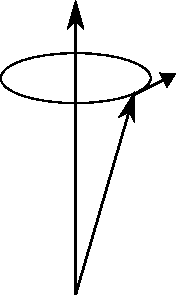
\includegraphics[width=0.7\textwidth]{Figures/Precessionv2}};
\node at (85pt,90pt) {\Large{$\mathbold{M}$}};
\node at (110pt,140pt) {\Large{$-\gamma\mathbold{M}\times\mathbold{H}$}};
\node at (20pt,150pt) {\Large{$\mathbold{H}$}};
\end{tikzpicture}
  \caption{}
\end{subfigure}%
\hspace{1cm}
\begin{subfigure}{.33\textwidth}
  \centering
  \begin{tikzpicture}
\node[above right] (img) at (0,0) {\includegraphics[width=0.6\textwidth]{Figures/DampedPrecessionv2}};
\node at (85pt,90pt) {\Large{$\mathbold{M}$}};
\node at (110pt,140pt) {\Large{$-\gamma\mathbold{M}\times\mathbold{H}$}};
\node at (-10pt,100pt) {\Large{$\alpha\mathbold{M}\times\partial_t\mathbold{M}$}};
\node at (20pt,150pt) {\Large{$\mathbold{H}$}};
\end{tikzpicture}
  \caption{}
\end{subfigure}
\caption{The precession of the magnetization vector around a magnetic field. In \textbf{(a)} the precession is undamped and so the magnetization performs counter-clockwise circular rotations around the magnetic field. In \textbf{(b)} the damping component pointing towards the magnetic field causes a spiralling motion of the magnetization vector that eventually aligns the magnetization with the magnetic field.}
\label{fig:Precessions}
\end{figure}
It should be noted that the magnetic field $\mathbold{H}$ that the magnetization precesses around is not only an external magnetic field applied to the system, but it is the effective magnetic field experienced locally by the magnetization. The direction of this magnetic field represents the direction in which the magnetization will have a minimum in the micromagnetic energy, and the effective field can therefore be written in terms of the micromagnetic energy. The effective field in the absence of an external field is given by
\begin{align}
\label{eq:EffectiveField}
\nonumber\mathbold{H}_{\textrm{eff}} &= -\frac{1}{\mu_0}\frac{\delta\epsilon[\mathbold{M}]}{\delta\mathbold{M}} \\
&= \frac{2A}{\mu_0M_s}\mathbold{\nabla}^2\mathbold{m}+\frac{2(K+\eta E)}{\mu_0M_s}m_z\mathbold{\hat{z}} + \frac{2D}{\mu_0M_s}\left(\frac{\partial m_z}{\partial x}\mathbold{\hat{x}}+\frac{\partial m_z}{\partial y}\mathbold{\hat{y}}-(\mathbold{\nabla}\cdot\mathbold{m})\mathbold{\hat{z}}\right),
\end{align}
with $\mathbold{m}$ being a unit vector in the direction of the magnetization. Here the symmetric exchange interaction, perpendicular and voltage induced magnetic anisotropy and interfacial DMI have been taken into consideration in the effective field.

Another thing to notice about the LLG equation is that only the direction of the magnetization $\mathbold{M}$ and not its magnitude changes with time. This can be seen by multiplying \eqref{eq:LLG} by $\mathbold{M}$ from the left:
\begin{align}
\mathbold{M}\cdot\frac{\textrm{d}\mathbold{M}}{\textrm{d}t} = \frac{1}{2}\frac{\textrm{d}}{\textrm{d}t} \mathbold{M}^2 =  \mathbold{M}\cdot\left(-\gamma\mathbold{M}\times\mathbold{H}+\frac{\alpha}{M_s}\mathbold{M}\times\frac{\textrm{d}\mathbold{M}}{\textrm{d}t}\right) = 0.
\end{align}
In other words the LLG equation conserves the magnitude of the magnetization, meaning $\frac{\textrm{d} M_s}{\textrm{d}t} = 0$.

\section{Spin-transfer torques}
The LLG equation presented in \eqref{eq:LLG} describes the dynamics of magnetic moments in the presence of external magnetic fields and internal effective fields that try to minimize the energy of the system. However, there are also other means of inducing dynamics of the magnetization in a material. The LLG equation can be extended to include these effects by adding torques to the right hand side of the equation (note that these torques will not have the same units as a mechanical torque, but the effect is well described by the term torque as it appears as a rotation of the magnetization direction). One method that has shown promise in inducing magnetization dynamics is the spin-transfer torque. In \cite{Berger1978} Berger noted that when you apply a current through a magnetic domain wall, the main effect was not a scattering of the electrons, but that the domain wall tended to follow the motion of the electrons. When a spin-polarized current is passing through a magnetic material, the conduction electrons will want to align their magnetic moments with the local magnetization in the material to reduce their energy. The way the electrons reach a lower energy state is by the torque acting on them from the local magnetization due to the fact that they are not aligned (or anti-aligned). Since the conduction electrons experience a torque when passing through a magnetization not parallel to their own magnetic moments, Newton's third law dictates that there must be an equal and opposite torque acting on the local magnetization. In other words, through a means of conserving angular momentum the conduction electrons transfer some of their spin to the local magnetization, hence the term spin-transfer torque (STT). Slonczewski introduced this torque in the LLG equation for the case of STT acting on a magnetic multilayer system \cite{Slonczewski1996}. This torque was observed experimentally a few years after the publications by Berger and Slonczewski \cite{Tsoi1998,Myers1999}.

\subsection{Adiabatic spin-transfer torque} \label{sec:AdSTT}
To start the introduction of spin-transfer torques we will first discuss them qualitatively in what is known as the adiabatic regime. In this regime it is assumed that the magnetic moments of the conduction electrons passing through the magnetic material relaxes fast enough to always follow the local magnetization. If we then consider a current passing through a magnetic layer with a magnetization direction $\mathbold{m}_i = \mathbold{M}_i/M_s$, the magnetic moment of the electrons will be parallel to $\mathbold{m}_i$. Not long after passing through $\mathbold{m}_i$, the electrons pass through another magnetic material with a magnetization direction $\mathbold{m}_j$ which is tilted with respect to $\mathbold{m}_i$. Since the electrons have a magnetic moment that is not aligned with $\mathbold{m}_j$, this magnetization will lead to a torque acting on the conduction electrons to make their magnetic moments relax to be aligned with $\mathbold{m}_j$ instead of $\mathbold{m}_i$. As we mentioned earlier, there is then an equal torque acting on $\mathbold{m}_j$ in the opposite direction, attempting to align it with the magnetic moment of the electrons, which is $\mathbold{m}_i$ at the time of incidence. If we then assume that the magnitude of $\mathbold{M}_i$ and $\mathbold{M}_j$ are equal, the torque acting on $\mathbold{m}_j$ must then be proportional to the component of $\mathbold{m}_i$ which is perpendicular to $\mathbold{m}_j$. This means that the torque is proportional to $\mathbold{m}_i-(\mathbold{m}_i\cdot\mathbold{m}_j)\mathbold{m}_j$, as illustrated in Figure \ref{fig:AdSTT}.
%\begin{figure}[h!]
%  \centering
%  \includegraphics[width=0.4\linewidth]{Figures/AdiabaticSTT}
%\caption{The adiabatic spin-transfer torque acting on a magnetic moment $\mathbold{m}_j$ from a spin-polarized current having passed through the magnetic moment $\mathbold{m}_i$ is proportional to the component of $\mathbold{m}_i$ perpendicular to $\mathbold{m}_j$.}
%\label{fig:AdSTT}
%\end{figure}

\begin{figure}[h!]
\centering
\begin{tikzpicture}
\node[above right] (img) at (0,0) {\includegraphics[width=0.4\textwidth]{Figures/AdiabaticSTTv2}};
\node at (5pt,110pt) {\Large{$\mathbold{m}_i$}};
\node at (120pt,60pt) {\Large{$\mathbold{m}_j$}};
\node at (150pt,140pt) {\textcolor{red}{\Large{$\mathbold{m}_i-\left(\mathbold{m}_i\cdot\mathbold{m}_j\right)\mathbold{m}_j$}}};
\end{tikzpicture}
        \caption{The adiabatic spin-transfer torque acting on a magnetic moment $\mathbold{m}_j$ from a spin-polarized current having passed through the magnetic moment $\mathbold{m}_i$ is proportional to the component of $\mathbold{m}_i$ perpendicular to $\mathbold{m}_j$.}
        \label{fig:AdSTT}
\end{figure}

This discussion was for two discrete magnetic moments. Let us now consider a case where the magnetization in a material varies slowly in a way that can be described by a function of position, such as a magnetic domain wall. We can still use the result from before, but instead of $\mathbold{m}_j$ being a magnetic moment in a direction independent of the direction of $\mathbold{m}_i$, there is only an infinitesimal change in $\mathbold{m}_j$ from $\mathbold{m}_i$. So when the electrons arrive at the magnetization at a position $x+\d x$ (here assuming the electrons flow in the positive $x$-direction), their magnetic moments are aligned with the magnetization at the position $x$. Since the magnetization varies slowly, we can do a Taylor expansion to approximate the magnetization at position $x+\d x$ as a function of the magnetization at position $x$:
\begin{align}
    \mathbold{m}(x+\d x) \approx \mathbold{m}(x) + \d x\partial_x \mathbold{m}(x).
\end{align}
Typically $\d x$ would be on the length scale of the lattice constant. Using this expansion we can then find the direction of the torque acting on the magnetization at $x+\d x$ from the current which has a polarization along the magnetization at $x$:
\begin{align}
\nonumber&\hspace{5.5mm}\mathbold{m}(x)-\left[\mathbold{m}(x)\cdot\mathbold{m}(x+\d x)\right]\mathbold{m}(x+\d x) \\
\nonumber&\approx \mathbold{m}(x)-\left[1 + \d x \mathbold{m}(x)\cdot\partial_x \mathbold{m}(x)\right]\left[\mathbold{m}(x) + \d x\partial_x \mathbold{m}(x)\right] \\
&= -\d x \partial_x \mathbold{m}(x). \label{eq:DiffSTTterm}
\end{align}
Here we have used that $\mathbold{m}(x)\cdot\partial_x \mathbold{m}(x) = 0$ as the magnitude of $\mathbold{M}(x)$ is assumed to be constant for all positions. As we can see the result is somewhat different than for the two discrete magnetic moments as we have a differential in the torque, but the physical interpretation of the result is still the same. When the magnetic moments of the conduction electrons follow the local magnetization, their magnetic moment is adjusted from $\mathbold{m}(x)$ to $\mathbold{m}(x) + \d x \partial_x \mathbold{m}(x)$. The direction of the torque acting on the magnetization at $x +\d x$ must then be in the opposite direction of this change, along $-\d x \partial_x \mathbold{m}(x)$. Remember that what we have discussed so far has only been the direction of the torque acting on the local magnetization, and not its magnitude. A pre-factor must then be included that reflects how much spin is transferred from each electron to the local magnetization, the frequency of each electron passing through the magnetization, and how many of these electrons that are polarized of the magnetization at the previous position. Each electron has a magnetic moment $\mathbold{\mu} = \mu_B \mathbold{m}$, with $\mathbold{m}$ being a unit vector in the direction of the magnetization. The frequency of the electrons passing through the magnetization can be expressed in terms of the current, and since the magnetization is a volume average of the magnetic moments in the material, we want the current density to describe the rate of change to the magnetization. Letting the current passing through per cross-sectional area be $j$, the current density is $j/d_j$ with $d_j$ being the thickness of the material with magnetization $\mathbold{M}_j$. Assuming a portion $P$ of the electrons in the current are polarized, the frequency of each electron transferring its magnetic moment to the magnetic material per volume unit is $jP/(-ed)$, where we have divided the current by its charge carrier. The adiabatic spin-transfer torque acting on a magnetization $\mathbold{M}_j$ after a current passing through a magnetization $\mathbold{M}_i$ is then
\begin{align}
    \mathbold{T}_{\text{STT}}^{\textrm{(adiabatic)}} = -\frac{\mu_B j P}{e d_j} (\mathbold{m}_i-(\mathbold{m}_i\cdot\mathbold{m}_j)\mathbold{m}_j)
    = -\frac{\gamma \hbar jP}{2 e \mu_0 d}\mathbold{m}_j\times\left(\mathbold{m}_i\times\mathbold{m}_j\right).
    \label{eq:STT_Adiabatic_Macro}
\end{align}
In a material with a slowly varying magnetization, the thickness of the magnetization goes from $d_j$ to $\d x$. Using the expression found in \eqref{eq:DiffSTTterm} and that the current is moving in the direction $\mathbold{\hat{j}}$, the adiabatic STT in this case becomes
\begin{align}
 \mathbold{T}_{\text{STT}}^{\textrm{(adiabatic)}} = \frac{\mu_B j P}{e M_s} (\mathbold{\hat{j}}\cdot\mathbold{\nabla})\mathbold{M}(\mathbold{r}). \label{eq:AdSTTnonuniform}
\end{align}
These torques can then be included in the right hand side of the LLG equation in \eqref{eq:LLG} to describe the dynamics of adiabatic STTs.

\subsection{General spin-transfer torque} \label{sec:GeneralSTT}
So far we have discussed how STT terms would appear in the LLG equation if the magnetic moments of the conduction electrons follow the local magnetization adiabatically. We will now derive the STT terms for a slowly varying magnetization more rigidly based on the spin continuity equation. This will be done for a more general case where the magnetic moments of the conduction electron can have a small component perpendicular to the local magnetization. This derivation mainly follows the derivation by Zhang and Li \cite{ZhangLi-04}. We start by considering the spin continuity equation. This is based on the continuity equation for an arbitrary quantity $\rho$,
\begin{align}
\partial_t\rho + \mathbold{\nabla}\hat{J}_{\rho} = 0,
\end{align}
with $\hat{J}_{\rho}$ being the current of the quantity $\rho$. This continuity equation assumes that the quantity $\rho$ is conserved, but this is not the case for the spins in our system. The spins of the conduction electrons interact with the local magnetization, and in addition they can be scattered by the material. To reflect this we introduce sources and sinks on the right hand side of the continuity equation, so that it is given by
\begin{align}
\partial_t\mathbold{s} + \mathbold{\nabla}\hat{J} = \frac{1}{i\hbar} \left[\mathbold{s}, H_{sd}\right] - \mathbold{\Gamma}(\mathbold{s}).
\end{align}
Here $\mathbold{s}$ is the spin operator for the conduction electrons, $\hat{J}$ the spin-current operator, $\mathbold{\Gamma}(\mathbold{s})$ the relaxation rate of the conduction electrons due to scattering, and $H_{sd}$ the $s$-$d$ Hamiltonian
\begin{align}
H_{sd} = -J_{\textrm{ex}}\mathbold{s}\cdot\mathbold{S}
\end{align}
which describes the (anti)ferromagnetic coupling between the itinerant spins $\mathbold{s}$ and local spins $\mathbold{S}$ depending on the sign of the coupling strength $J_{\textrm{ex}}$. In the micromagnetic model we are in a semi-classical limit, and we will therefore not treat the local spins quantum mechanically as operators, but as expectation values. The spins of the conduction electrons, however, we will still treat as operators for now. We proceed by calculating the commutator
\begin{align}
\left[\mathbold{s}, H_{sd}\right]_i = -J_{\textrm{ex}} \left[s_i, s_j S_j\right] = -J_{\textrm{ex}}\left[s_i, s_j\right] S_j.
\end{align}
Here we assume the Einstein summation convention. Note that $S_j$ can be pulled out of the commutators as it is not treated as an operator. The spin operators satisfy the commutation relation
\begin{align}
\left[s_i, s_j\right] = i\hbar\varepsilon_{ijk}s_k,
\end{align}
which can be obtained from the Pauli matrix commutation relation as $s_i = \hbar \sigma_i/2$. We then find that
\begin{align}
\frac{1}{i\hbar}\left[\mathbold{s}, H_{sd}\right] = -J_{\textrm{ex}}\mathbold{S}\times\mathbold{s}.
\end{align}
From now on we will also treat the remaining operators as expectation values. We make the ansatz that the spin density $\mathbold{m}$ of the conduction electrons are mainly parallel to the local magnetization $\mathbold{M}$, but allow a small perpendicular component $\delta\mathbold{m}$:
\begin{align}
    \mathbold{m} = \langle\mathbold{s}\rangle = \frac{m_0}{M_s} \mathbold{M} + \delta\mathbold{m}.
\end{align}
Note here that the ratio $m_0/M_s$ is very small, as the magnetization of the current is far below saturation. Moving on to the expectation value of the spin-current, we can write this as a tensor product between the velocity of the electrons, and their spin: $\langle\hat{J}\rangle = \mathbold{v}\otimes\mathbold{s}$. Instead of writing this expectation value in terms of the velocity $\mathbold{v}$ and spin $\mathbold{s}$, we want to write it in terms of the current density and magnetization. Using that $\mathbold{s} \approx \mu_B\mathbold{M}/M_s$ and following a similar approach as in the last section to rewrite the velocity in terms of the current $j$ per unit area, we find that
\begin{align}
\langle\hat{J}\rangle = -\frac{\mu_B P}{eM_s} \mathbold{j}\otimes\mathbold{M}.
\end{align}
Note that here we have assumed the spin current is adiabatic. To be exact one needs to include a non-adiabatic spin-current term $\delta\langle\hat{J}\rangle$, but it is assumed this is negligible. The product $\mathbold{\hat{\nabla}}\langle\hat{J}\rangle$ in the spin continuity equation then becomes
\begin{align}
\mathbold{\hat{\nabla}}\langle\hat{J}\rangle = -\frac{\mu_B P}{e M_s}\left(\mathbold{j}\cdot\mathbold{\nabla}\right)\mathbold{M}
\end{align}
when one assumes a uniform charge current density $\mathbold{j}$. Lastly, we approximate the relaxation rate due to scattering $\mathbold{\Gamma}(\mathbold{s})$ by the expectation value 
\begin{align}
\langle\mathbold{\Gamma}(\mathbold{s})\rangle \approx \frac{\delta\mathbold{m}}{\tau_{\textrm{sf}}},
\end{align}
with $\tau_{\textrm{sf}}$ being the spin-flip relaxation time. The spin continuity equation then becomes
\begin{align}
\partial_t\mathbold{m} -\frac{\mu_B P}{e M_s}\left(\mathbold{j}\cdot\mathbold{\nabla}\right)\mathbold{M} =   -\frac{J_{\textrm{ex}} S}{M_s}\mathbold{m}\times\mathbold{M} - \frac{\delta\mathbold{m}}{\tau_{\textrm{sf}}} =    -\frac{1}{\tau_{\textrm{ex}}M_s}\delta\mathbold{m}\times\mathbold{M} - \frac{\delta\mathbold{m}}{\tau_{\textrm{sf}}} \label{eq:SpinContinuityEq}
\end{align}
where we have introduced the spin relaxation $\tau_{\textrm{ex}} = (J_{\textrm{ex}}S)^{-1}$ time due to the exchange interaction. This is a time-scale that indicates how fast the spins of the conduction electrons align with the local spins, and this time-scale becomes smaller the stronger the exchange interaction ($\sim J_{\text{ex}}$) is. The first term appearing on the right hand side is a torque acting on the spin of the electrons due to an interaction with the local magnetization. As we have discussed earlier, Newton's third law then dictates that there must be an equal torque acting on $\mathbold{M}$ in the opposite direction, leaving us with the spin-transfer torque
\begin{align}
\mathbold{T}_{\text{STT}} = \frac{1}{\tau_{\textrm{ex}}M_s}\delta\mathbold{m}\times\mathbold{M}.
\end{align}
To determine this torque we must first find $\delta\mathbold{m}$. We can do this based on \eqref{eq:SpinContinuityEq}, but first we find an expression for $\delta \mathbold{m} \times \mathbold{M}$, which we can obtain by taking the cross product of \eqref{eq:SpinContinuityEq} with $\mathbold{M}$ from the right. We then find that
\begin{align}
\delta\mathbold{m}\times\mathbold{M} = \tau_{\textrm{sf}}\left[\frac{m_0}{M_s}\mathbold{M}\times\partial_t\mathbold{M} - \frac{\mu_B P}{e M_s} \mathbold{M}\times(\mathbold{j}\cdot\mathbold{\nabla})\mathbold{M} + \frac{M_s}{\tau_{\textrm{ex}}}\delta\mathbold{m} \right]
\end{align}
where we have neglected the time derivative of $\delta\mathbold{m}$. Inserting the expression for $\delta\mathbold{m}$ from \eqref{eq:SpinContinuityEq} into the expression above, we finally find that the total spin-transfer torque becomes
\begin{align}
\mathbold{T}_{\text{STT}} = \frac{1}{1+\beta^2} \left[ \frac{\beta m_0}{M_s^2}\mathbold{M}\times\partial_t\mathbold{M} - \frac{m_0}{M_s} \partial_t\mathbold{M} + \frac{\mu_B P}{e M_s} (\mathbold{j}\cdot\mathbold{\nabla})\mathbold{M} - \frac{\beta \mu_B P}{e M_s^2} \mathbold{M}\times(\mathbold{j}\cdot\mathbold{\nabla})\mathbold{M}\right],
\end{align}
where we have introduced the ratio $\beta = \tau_{\textrm{ex}}/\tau_{\textrm{sf}}$. The first two terms on the right hand side are on a form that already appear in the LLG equation, and introduce no new physics. In addition, they are proportional to $m_0/M_s$, and are therefore negligible. The third term we recognize being the adiabatic STT term in \eqref{eq:AdSTTnonuniform} that we found in the previous section, with an additional factor $(1+\beta^2)^{-1}$. The last term is of particular interest, as it is on a form that we have not seen before. As we can see, the term is perpendicular to the adiabatic STT and contains an additional factor $\beta$. In the adiabatic regime, which we considered in the previous section, $\beta \rightarrow 0$ as the spin-flip relaxation time is much greater than the exchange relaxation time when the conduction electrons follow the local magnetization adiabatically. The last term therefore only appears when we are not in the adiabatic regime, and is therefore called the non-adiabatic STT. This torque, which is caused by the magnetic moments of the itinerant electrons that are not aligned with the local magnetization, will twist the magnetization out of the plane spanned by the magnetization in that area. 